
\subsubsection{Distribution of Small Structures}
For smaller structures, we can observe that they not only predicted less accurately but are generally less present. figure \ref{fig:high-modes}

\begin{figure}[h]
    \centering
    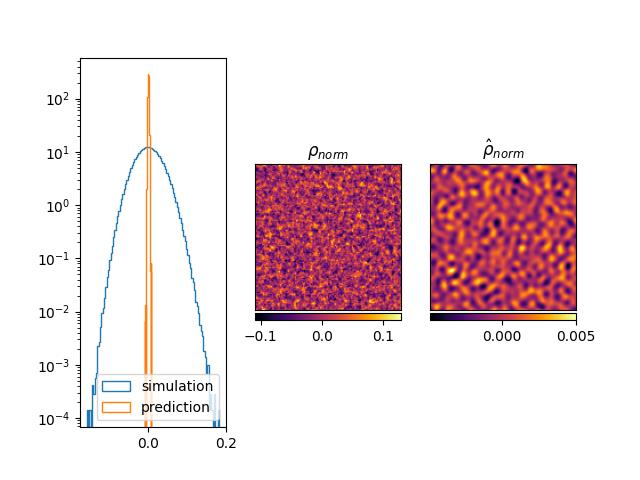
\includegraphics[width=0.5\linewidth]{high_modes.jpg}
    \caption{Enter Caption}
    \label{fig:high-modes}
\end{figure}


\subsection{IC Particle Velocities}

Once we have the displacement field, we can now compute the velocities using the formulate

\begin{equation}
    \mathbf{v} = \frac{d D_+(a)}{d a} \cdot \mathbf{s}(\mathbf{q}).
\end{equation}

where $\frac{d D_+(a)}{d a}$ can be approximated by

\begin{equation}
    D_+(a) = \frac{\frac{5}{2} \Omega_M}{
    \Omega_m^{\frac{4}{7}} - \Omega_{\Lambda} + ( 1 + \frac{\Omega_m}{2})(1 + \frac{\Omega_{\Lambda}}{70})
    }.
    \label{eq:growth_da}
\end{equation}



\section{IC Generation}
\label{IC-Gen}

To understand the common method for generating initial conditions, we have implemented the approach in Python. Our goal is to transform a random density field, as seen in Figure \ref{fig:random}, where the power spectrum is more or less constant, into one with an arbitrary power spectrum, defined in our case by a sine wave, as shown on the right of the figure.

\begin{figure}[h]
    \centering
    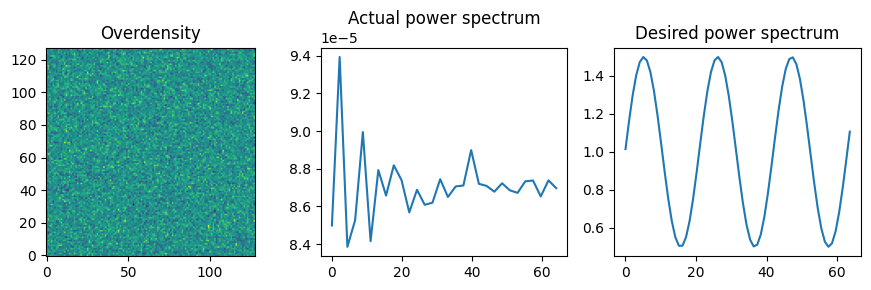
\includegraphics[width=0.75\linewidth]{match_ps.png}
    \caption{Random distribution, its power spectrum, and the desired power spectrum.}
    \label{fig:random}
\end{figure}

According to Pen et al. (1997), we need to compute the correlation kernel \citep{}

\begin{equation}
    A(k) = \sqrt{P(k)}.
\end{equation}

As depicted in Figure \ref{fig:correlation-kernel}, the process involves several steps including transforming noise in Fourier space, applying the correlation kernel, and eventually returning to real space.

\begin{figure}[h]
    \centering
    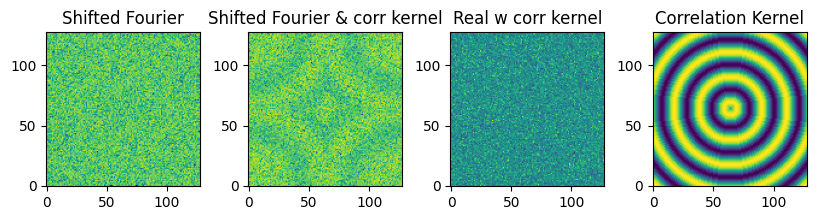
\includegraphics[width=0.75\linewidth]{2.png}
    \caption{From left to right: Noise in shifted Fourier space, noise with the correlation kernel applied in shifted Fourier space, noise with the correlation kernel applied in real space, and the correlation kernel in Fourier space.}
    \label{fig:correlation-kernel}
\end{figure}

\begin{figure}[h]
    \centering
    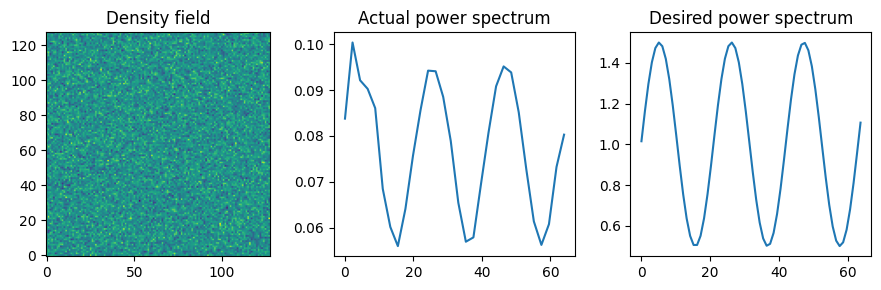
\includegraphics[width=0.75\linewidth]{match_ps_3.png}
    \caption{The power spectrum of the resulting density field and the desired power spectrum.}
    \label{fig:result}
\end{figure}


We then convolve the white noise with the correlation kernel in Fourier space to generate the density field with the desired power spectrum:

\begin{equation}
    \delta(\mathbf{k}) = n(\mathbf{k}) A(\mathbf{k}).
\end{equation}

One potentially confusing aspect is that while we are looking for a 3D correlation kernel, our power spectrum is a scalar function of distance. However, we generate a correlation kernel where the real-valued variable \(k\) is defined as \(k = \sqrt{\mathbf{k}_x^2 + \mathbf{k}_y^2 + \mathbf{k}_z^2}\). A more accurate definition is:

\begin{equation}
    A(\mathbf{k}) = \sqrt{P(\langle \mathbf{k} \rangle)}.
\end{equation}

The resulting power spectrum of the generated density field, compared to the desired power spectrum, is depicted in Figure \ref{fig:result}.


\newpage
\section{From Discrete Density Fields to Particles}
\label{back}

If in theory we have generated a satisfactory initial condition using a neural network, we need a method to convert the discrete density field back into particle positions and their respective velocities.
We are given a mass assignment scheme 

\begin{equation}
    \mathcal{A}\Bigl(\mathbf{X}(t_i), \mathbf{m}\Bigr) \colon \mathbb{R}^{3N} \times \mathbb{R}^{N} \rightarrow \mathbb{R}^{L^3},
\end{equation}

where $\mathbf{X}$ is the a tensor stacking all $N$ particle positions

\begin{equation}
    \mathbf{X}(t_i) = \begin{bmatrix}
        \mathbf{X}(0, t_i) \\
        \mathbf{X}(1, t_i) \\
        \dots  \\
        \mathbf{X}(N, t_i)
    \end{bmatrix},
\end{equation}

and $\mathbf{m}$ is the vector of all masses

\begin{equation}
    \mathbf{m}= \begin{bmatrix}
        \mathbf{m}(0) \\
        \mathbf{m}(1) \\
        \dots  \\
        \mathbf{m}(N)
    \end{bmatrix}.
\end{equation}

We can now formulate the the loss function

\begin{equation}
    L_{IC} = \sum_{\mathbf{y} \in \Omega} \Biggl(\mathcal{A}\Bigl(\mathbf{X}(t_0), \mathbf{m}\Bigr)(\mathbf{y}) - \rho(\mathbf{y})\Biggr)^2.
\end{equation}

In our case the mass vector $\mathbf{m}$ is fixed as the total mass is evenly distributed among the particles. If $\mathcal{A}$ is a differentiable function, we can obtain the gradient using automatic differentiation 

\begin{equation}
    \Delta = \frac{\partial L_{IC}}{\partial \mathbf{X}(t_0)}.
\end{equation}

Now we can leverage the Adam optimizer \citep{kingma2014adam} to optimize the initial conditions.
In our case we have used CIC mass assignment for $\mathcal{A}$. Note that any mass assignment scheme can be used, however it must be a differentiable. This is not the case in the nearest neighbour assignment scheme. The nearest neighbour scheme, assigns all the mass of each particle to the nearest grid cell, hence it is not possible to perturb the particle positions and see a small difference in the distribution, effectively generating non smooth gradients. In this case, the method to choose the initial guess for $\mathbf{X}$ is crucial. As seen before, we can generate intitial conditions using the formula

\begin{equation}
    \mathbf{x} = \mathbf{q} - D_{+}(a)\mathbf{s}(\mathbf{q}),
\end{equation}

whereas $\mathbf{q}$ are the Lagrangian position, which is essential a 3D grid with uniform distances. Therefore if we wish to find $\mathbf{x}$ with the above optimization algorithm, we must choose $\mathbf{X}$ to be a uniform grid. Then we also able to compute the Displacement map $\mathbf{s}$ by reforming the previous equation into

\begin{equation}
    \mathbf{s}(\mathbf{q}) = \frac{\mathbf{q} - \mathbf{x}}{D_{+}(a)}.
\end{equation}

In figure \ref{fig:field-fit} we can observe the accuracy of the method applied to arbitrary sample from the small dataset. The figure shows the difference between the predicted minus the actual density field divided by the standard deviation. Hence a maximum deviation of 0.004 out of 1 is equivalent to a maximum deviation of $0.4\%$.

\begin{figure}[h]
    \centering
    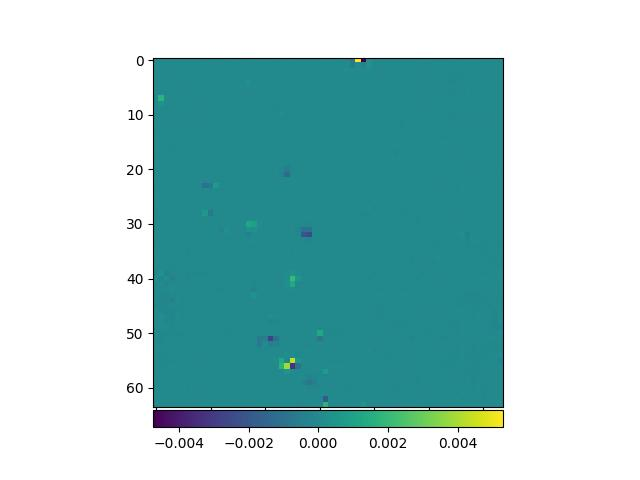
\includegraphics[width=0.5\linewidth]{cmp.jpg}
    \caption{Difference between fitted density field an actual density field normalized by dividing through the standard deviation.}
    \label{fig:field-fit}
\end{figure}

